% https://es.overleaf.com/latex/templates/project-report/jpzczmpsdzwm

%%% Preamble
\documentclass[paper=leter, fontsize=11pt]{scrartcl}
\usepackage[utf8]{inputenc}
\usepackage[spanish,mexico]{babel}
\usepackage[T1]{fontenc}    % use 8-bit T1 fonts
\usepackage{lmodern}
\usepackage{hyperref}       % hyperlinks
\usepackage{lipsum}
\usepackage[square,numbers]{natbib}

\usepackage[protrusion=true,expansion=true]{microtype}	
\usepackage{amsmath,amsfonts,amsthm} % Math packages
\usepackage[pdftex]{graphicx}
\usepackage{url}

\usepackage{tikz}

\usepackage{caption}
\usepackage{subcaption}

\usepackage{listings}
\lstdefinestyle{mystyle}{
    basicstyle=\ttfamily\footnotesize,
    breakatwhitespace=false,         
    breaklines=true,                 
    captionpos=b,                    
    keepspaces=true,                 
    numbers=left,                    
    numbersep=5pt,                  
    showspaces=false,                
    showstringspaces=false,
    showtabs=false,                  
    tabsize=4
}

\lstset{style=mystyle}
\renewcommand{\lstlistingname}{Código}

\graphicspath{ {img/} }

\selectlanguage{spanish}
\usepackage[spanish,onelanguage,ruled]{algorithm2e}


%%% Custom sectioning
\usepackage{sectsty}
\allsectionsfont{\centering \normalfont\scshape}


%%% Custom headers/footers (fancyhdr package)
\usepackage{fancyhdr}
\pagestyle{fancyplain}
\fancyhead{}											% No page header
\fancyfoot[L]{}											% Empty 
\fancyfoot[C]{}											% Empty
\fancyfoot[R]{\thepage}									% Pagenumbering
\renewcommand{\headrulewidth}{0pt}			% Remove header underlines
\renewcommand{\footrulewidth}{0pt}				% Remove footer underlines
\setlength{\headheight}{13.6pt}


%%% Equation and float numbering
\numberwithin{equation}{section}		% Equationnumbering: section.eq#
\numberwithin{figure}{section}			% Figurenumbering: section.fig#
\numberwithin{table}{section}				% Tablenumbering: section.tab#


%%% Maketitle metadata
\newcommand{\horrule}[1]{\rule{\linewidth}{#1}} 	% Horizontal rule

%%% https://tex.stackexchange.com/a/118217
\usepackage{mathtools}
\DeclarePairedDelimiter\ceil{\lceil}{\rceil}
\DeclarePairedDelimiter\floor{\lfloor}{\rfloor}

\usepackage{amsmath}

\title{
		%\vspace{-1in} 	
		\usefont{OT1}{bch}{b}{n}
		\normalfont \normalsize \textsc{Posgrado de Ingeniería de Sistemas} \\ [25pt]
		\horrule{0.5pt} \\[0.4cm]
		\huge Búsqueda en anchura y profundidad \\
		\horrule{2pt} \\[0.5cm]
}
\author{
		\normalfont 								\normalsize
        Alberto Benavides\\[-3pt]		\normalsize
        \today
}
\date{}


%%% Begin document
\begin{document}
\maketitle

\section{Introducción}

En grafos, se denomina \textit{búsqueda} a la operación de visitar nodos del grafo con la finalidad de encontrar un nodo específico. En el peor de los casos, se deben recorrer todos los nodos del grafo con una complejidad $\mathcal{O}(n)$ con la posibilidad de que el nodo de interés no sea encontrado. Estos algoritmos se utlizan cuando se desconoce la ubicación del nodo, en contraste con los algoritmos para colas prioritarias, por ejemplo , en que los montículos de Fibonacci permiten el acceso al menor elemento en tiempo $\mathcal{O}(n)$.

Para esta práctica se desarrollaron dos algoritmos de búsqueda, uno llamado \textit{búsqueda en profundidad} y el otro \textit{búsqueda en anchura}. Estos algoritmos fueron desarrollados en \texttt{javascript} con la ayuda de la librería \texttt{greuler} \cite{greuler} para mostrar una representación visual de los nodos.

\section{Definición de los algoritmos}

Ambos algoritmos comparten el principio de recorrer un grafo $G = (V, E)$ a partir de un vértice inicial $v \in V$, pero la manera de proceder es distinta en cada uno. Las búsquedas en anchura visitan nodo a nodo a través de las jerarquías inmediatas inferiores. Es decir, que tras partir del nodo inicial $n$, se busca primero en todos sus nodos vecinos $\{u, v\} in V_n$, posteriormente en todos los vecinos de los vecinos, y así sucesivamente. 

El algoritmo de búsqueda en profundidad explora los nodos extendiéndose en en camino de vecindades hasta agotarlo y luego regresa hasta algún camino no visitado para explorarlo a continuación, y se prosigue de este modo hasta que encuentra el nodo buscado o se visitan todos los nodos. 

\section{Árbol binario}

Con finalidades ilustrativas, se eligió como grafo una estructura de datos de \textit{árbol binario}. Estos árboles tienen la propiedad de que cuentan con un \textit{nodo inicial o raíz} a partir del cual se deben establecer hasta un máximo de dos vecindades. Por simplicidad, se suele denominar \textit{hijos} a los dos nodos que acompañan a otro nodo, a su vez nombrado \textit{padre}. Además, por ser dos los hijos, se les refiere como \textit{hijo izquierdo} e \textit{hijo derecho}. Esto puede verse en la imagen \ref{arbolBinarioSimple}.

\begin{figure}
    \centering
    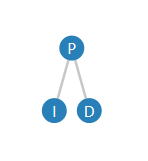
\includegraphics{arbolBinarioSimple.PNG}
    \caption{Representación de un árbol binario con tres nodos. La raíz o padre marcado por una P, el hijo izquierdo por una I y el derecho por una D.}
    \label{arbolBinarioSimple}
\end{figure}

La operación de inserción para un árbol binario se puede realizar de diversas maneras. En esta práctica se ha optado por utilizar un vector de nodos $N$ identificados cada uno por un índice $i \in {0, 1, 2, ...}$. Así, el nodo con índice $i = 0$ es el nodo raíz y para todos los demás nodos se asigna un entero consecutivo conforme al orden de la inserción. Los nodos con $i > 0$ son por defecto hijos de algún otro nodo con índice $j$ dado por \(j = \floor{(i - 1) / 2}\) en el entendido de que si $i \mod 2 = 0$ se trata del hijo derecho, mientras que en otro caso, es el hijo izquierdo.

\section{Implementaciones}

La búsqueda de un valor $k$ en anchura para un árbol binario definido de esta forma consiste en recorrer el vector de nodos como se muestra en el algoritmo \ref{algoritmoBusquedaAnchura}.

\begin{algorithm} %or another one check
	\SetAlgoLined
    \For{\(i \in N\)}{
        \If{\(n_i = v \)}{
            terminar\;
        }
    }
    \Return \(i\)

    \caption{Algoritmo de búsqueda en anchura.}
    \label{algoritmoBusquedaAnchura}
\end{algorithm}

En el caso del algoritmo de búsqueda en profunidad, se optó por una función recursiva que toma como parámetros el valor $k$ buscado y un nodo $m$ como se constata en el algoritmo \ref{algoritmoBusquedaProfundad}.
\begin{algorithm} %or another one check
	\caption{Algoritmo de búsqueda en profundidad.}
	\label{algoritmoBusquedaProfundad}
	\SetAlgoLined
    \SetKwFunction{FMain}{Profundidad}
    \SetKwProg{Fn}{Función}{:}{}
    \Fn{\FMain{$k$, $m$}}{
        \uIf{\(k = m\)}{
            \Return $\top$ \;
        }
        \Else{
            \(e \leftarrow \bot\) \;
            \If{\(\exists m_{\text{hijo izquierdo}}\)}{
                \texttt{Profundidad}($k, m_{\text{hijo izquierdo}}$) \;
            }
            \If{\(\exists m_{\text{hijo derecho}}\)}{
                \texttt{Profundidad}($k, m_{\text{hijo derecho}}$) \;
            } 
            \Return \( \bot \) \;
        }
        \Return \( \bot \) \;
    }
    \textbf{Fin Profundidad}

    \texttt{Produndidad}$(k, n)$\;
\end{algorithm}

Estas implementaciones pueden consultarse en \url{https://jbenavidesv87.github.io/algoritmos/search.html}.

\bibliographystyle{plainnat}
\bibliography{Biblio}

\end{document}